\documentclass{article}

\usepackage{amsmath}
\usepackage{amssymb}
\usepackage{bm}
\usepackage{CJKutf8}
\usepackage{color}
\usepackage{enumitem}
\usepackage{graphicx}
\usepackage{mathdots}
\usepackage{tikz}
\usepackage{wasysym}

\usetikzlibrary{snakes}

\allowdisplaybreaks

\begin{document}
\begin{CJK*}{UTF8}{gbsn}

\title{一些汇编的小坑}
\author{张艺瀚}
\date{}
\maketitle

\section{基本语法}

\begin{itemize}

\item
\verb|ADDR[BX][SI], ADDR[SI][BX], 0100H[BX][SI]|的寻址方式都是正确的。 \\

\item
一般来说,立即寻址只能用于源操作数寻址。 \\

\item
除源操作数为立即寻址的指令外,两个操作数的指令,其中必须有一个操作数的寻址方式为寄存器直接寻址。 \\
这样写是错误的:\verb|MOV BYTE PTR [DI], [SI]|。 \\

\item
在算术表达式中,除\verb|+, -, *, /|外,只能使用\verb|MOD|, \verb|SHL|, \verb|SHR|, \verb|AND|, \verb|OR|, \verb|XOR|, \verb|NOT|,它们在表达式中是作为逻辑算符存在的,表达式实在将源程序翻译成目标程序时求值的,而当它们出现在指令中时,要在执行目标程序时求值的。 \\

\item
\verb|SIZE|和\verb|LENGTH|只适用于\verb|DUP|分配的内存单元。 \\

\item
\verb|MOV AX, [0100H]|将被反汇编成\verb|MOV AX, 0100H|。 \\

\item
\verb|LEA|的目的操作数可以为任意16位通用寄存器或指针和变址寄存器,用\verb|LEA|指令获取偏移量和用\verb|OFFSET|算符获取偏移量的区别在于,\verb|OFFSET|只能跟标号。 \\
比如我们可以写:\verb|LEA AX, [BX + SI + 0100H]|, \\
但不能写:\verb|MOV AX, OFFSET [BX + SI + 0100H]|。 \\

\item
\verb|DS|, \verb|ES|, \verb|SS|中均可以存放指令,存放的是指令的编码,但不会被执行到,所以课本上说指令代码只能存在\verb|CS|中不能算错。如果想看指令编码可以反汇编,不要用这种反人类方式。 \\

\item
\verb|DEBUG|

\begin{itemize}
\item \verb|U|命令中可以给出两个地址,它们必须是偏移量。
\item \verb|T|命令格式:\verb|T [=地址] [,计数]|(可以指定步长)。
\item \verb|P|命令不进入\verb|CALL, INT|和循环。
\item \verb|R|后给出寄存器名称可以修改其值。
\item \verb|D|默认显示128字节内存,且可以给出的两个地址必须是偏移量。
\item \verb|A|命令下可以直接在指令中用偏移地址的值寻址,但将这些命令写到\verb|.ASM|文件中都是错的。 \\
如\verb|MOV AH, [0100H]|被翻译成\verb|MOV AH, 0100|,\verb|JMP 0100H|会报错。
\end{itemize}

\end{itemize}

\section{顺序结构}

\begin{itemize}

\item
\verb|MOV AX, LABEL|的写法是错误的。 \\

\item
\verb|ADD|, \verb|ADC|, \verb|SUB|, \verb|SBB|, \verb|CMP|, \verb|AND|, \verb|OR|, \verb|XOR|等指令的操作数中不得出现段寄存器。事实上,除传送指令,其他均不能用段寄存器。 \\

\item
\verb|MOV [BP + OFFSET DATA], AH|这种写法默认\verb|SS|寻址。 \\
\verb|MOV DATA[BP], AH|这种写法默认\verb|DS|寻址。将源程序翻译为目标程序时,翻译程序在\verb|DATA[BP]|前面自动加上\verb|DS:|。 \\

\item
对标志位的特殊影响
\begin{itemize}
\item \verb|NEG|操作前操作数非0,则操作后\verb|CF|置位,否则复位。
8位时的\verb|80H|,16位时的\verb|8000H|,\verb|NEG|后溢出,\verb|OF|被置位。
\item 执行\verb|MUL|后高位为0或执行\verb|IMUL|高位是低位符号位的扩展时(此时高位可丢弃),\verb|CF|, \verb|OF|被复位。 \\
另外,\verb|MUL|, \verb|IMUL|, \verb|DIV|, \verb|IDIV|源操作数不能为立即数。
\item \verb|DIV|, \verb|IDIV|不产生有效的标志位影响,各位不定。若溢出则产生0中断,结果不定。
\item \verb|CBW|, \verb|CWD|不影响标志位。
\item \verb|NOT|不影响标志位。 \\
\verb|AND|, \verb|OR|, \verb|XOR|, \verb|TEST|操作后,\verb|CF|, \verb|OF|被复位,除\verb|AF|不定外,其他位正常影响。
\item 移位操作后,最高位若改变则\verb|OF|被置位(只适用于移位1位的情况)。
\end{itemize}

\end{itemize}

\section{分支结构}

\begin{itemize}

\item
以下写法都是正确的:
\begin{itemize}
\item \verb| JMP LABEL |
\item \verb| JMP AX |
\item \verb| JMP MEM |
\end{itemize}

\verb|JMP [BX]|的写法是正确的,默认段间转移, \\
但写成:\verb|JMP WORD PTR [BX]|(段内转移)或\verb|JMP DWORD PTR [BX]|(段间转移)更好。 \\
但\verb|JMP 0100H|是错误的。 \\
对于\verb|JMP DWORD PTR [BX]|,\verb|BX|所值内存的低位的一个字存放偏移量,高位的一个字存放偏移量,届时前者被送入\verb|IP|,后者被送入\verb|CS|。 \\
\textcolor{red}{条件转移指令}后面\textcolor{red}{只能跟标号}。像\verb|JMP|那样的\verb|JC AX|, \verb|JC MEM|, \verb|JC [BX]|的写法统统错误。 \\
另外,如果要实现段间转移,\verb|LABEL|要在其他段中用\verb|PUBLIC|说明,在本段中用\verb|EXTRN|说明。 \\

\end{itemize}

\section{循环结构}

\begin{itemize}

\item
数据传最长64K。 \\

\item
\verb|MOVS|, \verb|MOVSB|, \verb|MOVSW|, \verb|CMPS|, \verb|CMPSB|, \verb|CMPSW|的两个操作数可均为存储器操作数。 \\
串操作指令操作数的写法:
\begin{itemize}
\item \verb| MOVS ES: DATA2, DS: DATA1 |
\item \verb| CMPS DS: DATA1, ES: DATA2 |
\item \verb| SCAS ES: DATA2 |
\item \verb| LODS DS: DATA1 |
\item \verb| STOS ES: DATA2 |
\end{itemize}
上述指令格式中,\verb|DS:|可省略,\verb|ES:|不可省略。因为默认DS段寻址。 \\

\item
串操作指令的执行情况:
\begin{itemize}
\item \verb|CMPS, CMPSB, CMPSW: DS: [SI] - ES: [DI]|
\item \verb|SCAS, SCASB, SCASW: AL / AX - ES: [DI]|
\item \verb|LODS, LODSB, LODSW: AL / AX| $\leftarrow$ \verb|DS: [SI]|
\item \verb|STOS, STOSB, STOSW: ES: [DI]| $\leftarrow$ \verb|AL / AX|
\end{itemize}
\verb|MOVS|, \verb|MOVSB|, \verb|MOVSW|, \verb|CMPS|, \verb|CMPSB|, \verb|CMPSW|, \verb|LODS|, \verb|LODSB|, \verb|LODSW|, \verb|STOS|, \verb|STOSB|, \verb|STOSW|不影响标志位。 \\
使用串操作指令时可能需要预设的内容:
\begin{itemize}
\item \verb|DF|
\item \verb|SI|, \verb|DI|
\item \verb|CX|
\item \verb|AL / AX|
\end{itemize}

\item
\verb|LOOP|, \verb|LOOPE|, \verb|LOONE|指令与循环入口的距离为-126~129字节。其后\textcolor{red}{只能跟标号},像\verb|JMP|那样的\verb|LOOP AX|, \verb|LOOP MEM|, \verb|LOOP [BX]|的写法统统错误。这些指令不影响标志位。所以先将\verb|CX|减1再无条件转移到循环入口和直接\verb|LOOP|是有区别的。 \\

\item
\verb|REP|: 先判断\verb|CX|状态,再执行,再将\verb|CX|减1。 \\
\verb|LOOP|: 先执行,再将\verb|CX|减1,再判断\verb|CX|状态。 \\
所以若将\verb|CX|置0,\verb|REP|修饰的指令执行0次,\verb|LOOP|执行65536次。 \\

\end{itemize}

\section{子程序}

\begin{itemize}

\item
用\verb|PROC|定义的子过程中不能使用\verb|HLT|等引起停机的指令。 \\

\item
以下写法都是正确的:
\begin{itemize}
\item \verb|CALL PN|
\item \verb|CALL AX|
\item \verb|CALL MEM|
\end{itemize}
只写\verb|CALL PN|,不标明\verb|NEAR|或\verb|FAR|,默认近调用。 \\
\verb|CALL [BX]|的写法是正确的,默认调用近过程,但这是做死的,强烈建议写成:\verb|CALL WORD PTR [BX]|(调用近过程)或\verb|CALL DWORD PTR [BX]|(调用远过程)。 \\
\verb|MEM|若为WORDL类型,则为近调用,若为\verb|DWORD|类型,则为远调用。 \\

\item
产生远调用时:
\begin{itemize}
\item \verb|CS|压栈
\item 低字所存偏移量送\verb|CS|
\item \verb|IP|压栈
\item 高字所存段地址送\verb|IP|
\end{itemize}
产生近调用时,没有前两步。 \\

\item
远调用不能用段寄存器指定入口。 \\
\end{itemize}

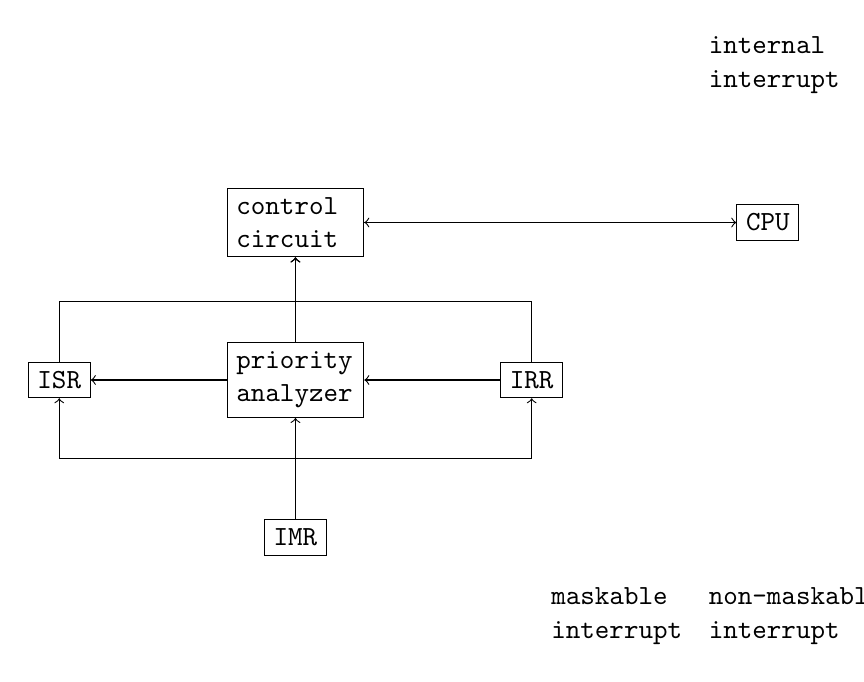
\begin{tikzpicture}
\path	(-3, 0)	node(isr)					[rectangle, draw]						{\verb|ISR|}
		(0, 0)	node(priority_analyzer)		[rectangle, draw, text width = 1.5cm]	{\verb|priority| \verb|analyzer|}
		(3, 0)	node(irr)					[rectangle, draw]						{\verb|IRR|}
		(0, 2)	node(control_circuit)		[rectangle, draw, text width = 1.5cm]	{\verb|control| \verb|circuit|}
		(0, -2)	node(imr)					[rectangle, draw]						{\verb|IMR|}
		(6, 2)	node(cpu)					[rectangle, draw]						{\verb|CPU|}
		(4, -3)	node(mi)					[text width = 1.5cm]					{\verb|maskable| \verb|interrupt|}
		(6, -3)	node(nmi)					[text width = 1.5cm]					{\verb|non-maskable| \verb|interrupt|}
		(6, 4)	node(internal_interrupt)	[text width = 1.5cm]					{\verb|internal| \verb|interrupt|};



\draw[->]	(isr.north)					|- (-1, 1) -|			(control_circuit);
\draw[->]	(priority_analyzer.north)	--						(control_circuit);
\draw[->]	(irr.north)					|- (1, 1) -|			(control_circuit);
\draw[->]	(imr.north)					|- (-1, -1) -|			(isr);
\draw[->]	(imr.north)					--						(priority_analyzer);
\draw[->]	(imr.north)					|- (1, -1) -|			(irr);

\draw[->]	(control_circuit.east)		--						(cpu.west);
\draw[->]	(cpu.west)					--						(control_circuit.east);

\draw[->]	(irr.west)					--						(priority_analyzer);
\draw[->]	(priority_analyzer.west)	--						(isr);
\end{tikzpicture}

\end{CJK*}
\end{document}